\section{Lab 4: Preemptive Multitasking}

\subsection{实验简介}

在本实验中,你将会实现抢占式多进程管理。需要哈工大操作系统课第五章的知识。

在第一部分里,需要向JOS添加多核支持,实现转轮调度,并添加基础的系统调用(用于添加或删除运行上下文环境,申请或对应内存)。

在第二部分里,需要实现Unix风格的fork()函数,支持从用户态环境建立一个自己的拷贝。

最后在第三部分里,需要添加对进程间通信(IPC)的支持,允许不同的用户态环境减间的交流并同步。还需要添加对硬件时钟中断和抢占的支持。

\subsection{实验目的}

\begin{itemize}
\item 了解并实现抢占式多进程管理
\item 了解并实现转轮法调度算法
\end{itemize}

\subsection{实验内容}

\subsubsection{准备工作}

需要用git commit把Lab3的成果提交,然后在lab3分支上新建分支lab4,并合并远程分支lab4。

\begin{figure}[H]
  \centering
  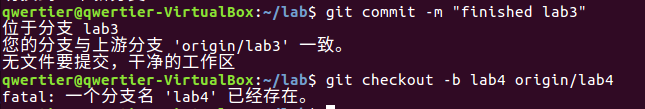
\includegraphics[width=6in]{figures/lab4/git_commit.png}
  \caption{使用git的截图}\label{fig:lab1:git_commit}
\end{figure}

\begin{ExerciseList}

\setcounter{Exercise}{0}

\subsubsection[第一部分: 多处理器支持及协作式多任务]{第一部分: 多处理器支持\footnote{Multiprocessor Support}及协作式多任务\footnote{Cooperative Multitasking} }

协作式多进程(Cooperative)指的是:进程主动(定期或者空闲时候)让出CPU的执行时间给其他进程来执行,这种模式非常依赖于程序的设计,如果程序写的很差, 进程长时间占用CPU的执行时间(大量计算密集型的操作或者等待外设等),这会让其他进程没有机会执行,从而造成整个操作系统失去响应。

协作式多任务在早期的操作系统中使用得比较广泛(比如Windows 9x、Classic Mac OS等等)。

我们将使JOS支持“对称多处理”(SMP),这是一种多处理器模型,其中所有的CPU都可以访问系统资源,例如内存和I / O总线。虽然所有的CPU在功能上与SMP完全相同,但在引导过程中,它们可以分为两种类型:引导处理器(BSP)负责初始化系统和引导操作系统; 并且只有在操作系统启动并运行之后,应用处理器(AP)才由BSP激活。BSP的处理器是由硬件和BIOS决定的。到目前为止,所有现有的JOS代码已经在BSP上运行。

在SMP系统中,每个CPU都有一个附带的本地APIC(LAPIC)单元。LAPIC单元负责在整个系统中提供中断。LAPIC还为连接的CPU提供唯一的标识符。在这个实验中,我们利用了LAPIC单元的下列基本功能(在kern / lapic.c中):

\begin{itemize}
\item 读取LAPIC标识符(APIC ID),以告知我们的代码当前正在哪个CPU上运行(请参阅cpunum())。
\item 发送STARTUP从BSP到的AP间中断(IPI)带来的其他CPU。
\item 在C部分,我们编程LAPIC的内置定时器来触发时钟中断,以支持抢先式多任务处理(请参阅参考资料 apic\_init())。
\end{itemize}

\Exercise{实现kern/pmap.c文件中的mmio\_map\_region函数。想要看它是如何被用到的,需要看kern/lapic.c中的lapic\_init。}

\begin{minted}{C}
void *
mmio_map_region(physaddr_t pa, size_t size)
{
    // Where to start the next region.  Initially, this is the
    // beginning of the MMIO region.  Because this is static, its
    // (just like nextfree in boot_alloc).
    static uintptr_t base = MMIOBASE;

    // Reserve size bytes of virtual memory starting at base and
    // map physical pages [pa,pa+size) to virtual addresses
    // [base,base+size).  Since this is device memory and not
    // regular DRAM, you'll have to tell the CPU that it isn't
    // safe to cache access to this memory.  Luckily, the page
    // tables provide bits for this purpose; simply create the
    // mapping with PTE_PCD|PTE_PWT (cache-disable and
    // write-through) in addition to PTE_W.  (If you're interested
    // in more details on this, see section 10.5 of IA32 volume
    // 3A.)
    //
    // Be sure to round size up to a multiple of PGSIZE and to
    // handle if this reservation would overflow MMIOLIM (it's
    // okay to simply panic if this happens).
    //
    // Hint: The staff solution uses boot_map_region.
    //
    // Your code here:
    int nextbase = ROUNDUP(base + size, PGSIZE);
    if (nextbase >= MMIOLIM) {
            panic("nextbase >= MMIOLIM");
    }
    boot_map_region(kern_pgdir, base, size, pa, PTE_PCD | PTE_PWT | PTE_W);

    void *ret = (void *)base;
    base = nextbase;

    return ret;
    // panic("mmio_map_region not implemented");
}
\end{minted}

在启动AP之前,BSP应首先收集有关多处理器系统的信息,例如CPU的总数,APIC ID和LAPIC单元的MMIO地址。kern / mpconfig.c中的mp\_init()函数 通过读取驻留在BIOS的内存区域中的MP配置表来检索此信息。

\Exercise{阅读kern/init.c中的boot\_aps()和mp\_main()函数,以及kern/mpentry.S文件。确保你理解了AP启动时的控制流。修改你在kern/pmap.c中的page\_init()的实现来防止添加MPENTRY\_PADDR位置的页到free list,以让我们可以安全的拷贝并在那个物理地址执行AP运行代码。你的代码应该通过check\_page\_free\_list()测试,但是可能通不过check\_kern\_pgdir()测试,这个我们稍后会修正。}

\begin{minted}{C}
// Setup code for APs
void
mp_main(void)
{
    // We are in high EIP now, safe to switch to kern_pgdir
    lcr3(PADDR(kern_pgdir));
    cprintf("SMP: CPU %d starting\n", cpunum());

    lapic_init();
    env_init_percpu();
    trap_init_percpu();
    xchg(&thiscpu->cpu_status, CPU_STARTED); // tell boot_aps() we're up

    // Now that we have finished some basic setup, call sched_yield()
    // to start running processes on this CPU.  But make sure that
    // only one CPU can enter the scheduler at a time!
    //
    // Your code here:

    lock_kernel();  // 锁定内核
    sched_yield();  // 调用轮换调度算法

    // Remove this after you finish Exercise 4
    // for (;;);
}
\end{minted}

编写多处理器操作系统时,区分CPU私有状态\footnote{per-CPU state}以及全局状态\footnote{global state}。需要了解如下部分:

\begin{itemize}
\item CPU独立内核栈\footnote{Per-CPU kernel stack}
\item Per-CPU TSS(Task State Segment)和TSS描述符
\item Per-CPU 当前环境指针
\item Per-CPU 系统寄存器
\end{itemize}

\Exercise{修改kern/pmap.c中的mem\_init\_mp()函数,来映射在KSTACKTOP位置的CPU独立栈。每个栈大小是KSTKSIZE字节加上KSTKGAP字节。代码需要通过check\_kern\_pgdir()测试。}

\begin{minted}{C}
void
mem_init_mp(void)
{
    // Map per-CPU stacks starting at KSTACKTOP, for up to 'NCPU' CPUs.
    //
    // For CPU i, use the physical memory that 'percpu_kstacks[i]' refers
    // to as its kernel stack. CPU i's kernel stack grows down from virtual
    // address kstacktop_i = KSTACKTOP - i * (KSTKSIZE + KSTKGAP), and is
    // divided into two pieces, just like the single stack you set up in
    // mem_init:
    //     * [kstacktop_i - KSTKSIZE, kstacktop_i)
    //          -- backed by physical memory
    //     * [kstacktop_i - (KSTKSIZE + KSTKGAP), kstacktop_i - KSTKSIZE)
    //          -- not backed; so if the kernel overflows its stack,
    //             it will fault rather than overwrite another CPU's stack.
    //             Known as a "guard page".
    //     Permissions: kernel RW, user NONE
    //
    // LAB 4: Your code here:

    int i;
    for (i=0; i<NCPU; i++) {
        boot_map_region(kern_pgdir,
                KSTACKTOP - i * (KSTKSIZE + KSTKGAP) - KSTKSIZE,  // 起始地址
                KSTKSIZE,                                         // 内存块大小
                PADDR(percpu_kstacks[i]),
                PTE_W|PTE_P);
    }
}
\end{minted}

\Exercise{kern/trap.c文件中trap\_init\_percpu()的代码初始化了TSS和TSS描述符。在Lab3中可以正常工作,但是在其他CPU上运行时就会出问题。修改这些代码已让它能运行在所有CPU上。}

\begin{minted}{C}
void
trap_init_percpu(void)
{
        // The example code here sets up the Task State Segment (TSS) and
        // the TSS descriptor for CPU 0. But it is incorrect if we are
        // running on other CPUs because each CPU has its own kernel stack.
        // Fix the code so that it works for all CPUs.
        //
        // Hints:
        //   - The macro "thiscpu" always refers to the current CPU's
        //     struct CpuInfo;
        //   - The ID of the current CPU is given by cpunum() or
        //     thiscpu->cpu_id;
        //   - Use "thiscpu->cpu_ts" as the TSS for the current CPU,
        //     rather than the global "ts" variable;
        //   - Use gdt[(GD_TSS0 >> 3) + i] for CPU i's TSS descriptor;
        //   - You mapped the per-CPU kernel stacks in mem_init_mp()
        //
        // ltr sets a 'busy' flag in the TSS selector, so if you
        // accidentally load the same TSS on more than one CPU, you'll
        // get a triple fault.  If you set up an individual CPU's TSS
        // wrong, you may not get a fault until you try to return from
        // user space on that CPU.
        //
        // LAB 4: Your code here:

        // Setup a TSS so that we get the right stack
        // when we trap to the kernel.
        thiscpu->cpu_ts.ts_esp0 = KSTACKTOP - cpunum() * (KSTKSIZE + KSTKGAP);
        thiscpu->cpu_ts.ts_ss0 = GD_KD;

        // Initialize the TSS slot of the gdt.
    gdt[(GD_TSS0 >> 3) + cpunum()] = SEG16(STS_T32A,
                                           (uint32_t) &thiscpu->cpu_ts,
                                           sizeof(struct Taskstate) - 1,
                                           0);
    gdt[(GD_TSS0 >> 3) + cpunum()].sd_s = 0;

        // Load the TSS selector (like other segment selectors, the
        // bottom three bits are special; we leave them 0)
        //ltr(GD_TSS0 + cpunum()*sizeof(struct Segdesc));
    ltr(((GD_TSS0 >> 3) + cpunum()) << 3);

        // Load the IDT
    lidt(&idt_pd);
}
\end{minted}

如图\ref{fig:lab4:mcpu},四个CPU都正常初始化。

\begin{figure}[H]
  \centering
  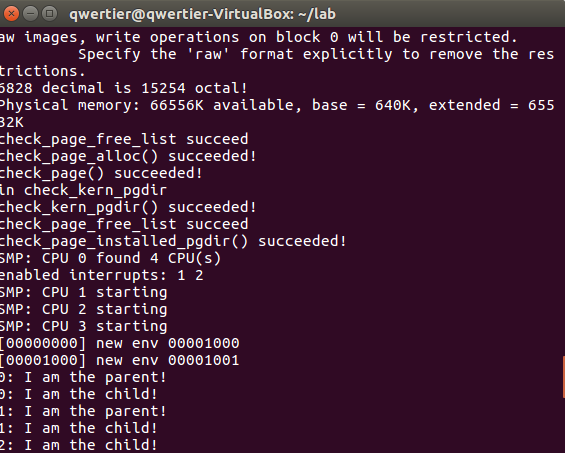
\includegraphics[width=6in]{figures/lab4/mcpu.png}
  \caption{QEMU启动截图}\label{fig:lab4:mcpu}
\end{figure}

我们当前的代码在mp\_main()函数中初始化AP之后就不会再运行了。在让AP继续运行前,我们首先需要解决竞争问题当多个CPU运行同一个内核时。最简单的方式是使用一个大内核锁。这个大内核锁是一个全局锁会作用于当进程进入内核模式时,而且在返回用户模式时会被释放。在这个模型下,用户模式下的进程可以在当前运行在任何可行的CPU上,但是不能有任何一个进程运行在内核模式中。

应该在四个位置应用大内核锁:

\begin{itemize}
\item 在i386\_init()BSP唤醒其他CPU之前获取锁。
\item 在mp\_main()初始化AP后获取锁,然后调用sched\_yield()该AP启动运行环境。
\item 在trap()从用户模式中获取锁时。要确定陷阱是发生在用户模式还是在内核模式下,请检查低位tf\_cs。
\item 在切换到用户模式之前env\_run(),立即释放锁定。不要太早或太晚,否则会遇到冲突。
\end{itemize}

\Exercise{如上所述,应用大内核锁,通过调用lock\_kernel()并unlock\_kernel()在适当的位置。}

只需要在i386\_init(), mp\_main(), trap()这几个函数中添加lock\_kernel(),在env\_run()中添加unlock\_kernel()即可。

因为前三个函数都是进入内核态,而最后的env\_run()是从内核态返回用户态。

\Exercise{在/kern/sched.c文件的sched\_yield()中实现轮转调度,不要忘记修改syscall()发送sys\_yield()。确保在mp\_main()中调用sched\_yield()。并修改kern/inic.c来创建所有运行程序user/yield.c。}

JOS的轮转调度算法如下:

\begin{enumerate}
\item 函数sched\_yield()在新的kern/sched.c中,负责选择一个进程来运行。envs[]以循环的方式按顺序搜索数组,在刚才运行的环境之后(或者在数组的开始处,如果没有以前运行的环境)开始,选择状态为ENV\_RUNNABLE(见inc/ env.h)的进程,并调用env\_run()进入该进程。
\item sched\_yield()决不能同时在两个CPU上运行相同的进程。它可以告诉一个环境当前正在某个CPU(可能是当前的CPU)上运行,因为该进程的状态将会是ENV\_RUNNING。
\item 已经实现了一个新的系统调用sys\_yield(),进程可以调用内核的sched\_yield()功能,从而自动放弃CPU到不同的进程。
\end{enumerate}

修改kern/sched.c的sched\_yield()函数:

\begin{minted}{C}
void
sched_yield(void)
{
        struct Env *idle;

        // Implement simple round-robin scheduling.
        //
        // Search through 'envs' for an ENV_RUNNABLE environment in
        // circular fashion starting just after the env this CPU was
        // last running.  Switch to the first such environment found.
        //
        // If no envs are runnable, but the environment previously
        // running on this CPU is still ENV_RUNNING, it's okay to
        // choose that environment.
        //
        // Never choose an environment that's currently running on
        // another CPU (env_status == ENV_RUNNING). If there are
        // no runnable environments, simply drop through to the code
        // below to halt the cpu.
        // LAB 4: Your code here.
        uint32_t envid = curenv? ENVX(thiscpu->cpu_env->env_id): -1;
        uint32_t first_eid = (++envid) % NENV;
        uint32_t next_envid;
        int i;

        // case: 进程可运行
        for (i = 0; i < NENV; i++) {
          next_envid = (first_eid+i) % NENV;
          if (envs[next_envid].env_status == ENV_RUNNABLE) {
            env_run(&envs[next_envid]);
            break;
          }
        }

        // case: 进程在运行
        if (curenv && curenv->env_status == ENV_RUNNING) {
          env_run(curenv);
        }

        // sched_halt never returns
        sched_halt();
}
\end{minted}

修改kern/inic文件的i386\_init()函数:

\begin{minted}{C}
void
i386_init(void)
{
        extern char edata[], end[];

        // Before doing anything else, complete the ELF loading process.
        // Clear the uninitialized global data (BSS) section of our program.
        // This ensures that all static/global variables start out zero.
        memset(edata, 0, end - edata);

        // Initialize the console.
        // Can't call cprintf until after we do this!
        cons_init();

        cprintf("6828 decimal is %o octal!\n", 6828);

        // Lab 2 memory management initialization functions
        mem_init();

        // Lab 3 user environment initialization functions
        env_init();
        trap_init();

        // Lab 4 multiprocessor initialization functions
        mp_init();
        lapic_init();

        // Lab 4 multitasking initialization functions
        pic_init();

        // Acquire the big kernel lock before waking up APs
        // Your code here:
        lock_kernel();

        // Starting non-boot CPUs
        boot_aps();

#if defined(TEST)
        // Don't touch -- used by grading script!
        ENV_CREATE(TEST, ENV_TYPE_USER);
#else
        // Touch all you want.
        //ENV_CREATE(user_primes, ENV_TYPE_USER);
        ENV_CREATE(user_dumbfork, ENV_TYPE_USER);
#endif // TEST*

        // Schedule and run the first user environment!
        sched_yield();
}
\end{minted}

尽管内核现在可以在多个用户级环境之间运行和切换,但仍然局限于运行内核最初设置的环境。现在将实现必要的JOS系统调用,以允许用户环境创建并启动其他新用户环境。

Unix提供fork()系统调用作为其进程创建原语。Unix fork()复制调用进程(父进程)的整个地址空间来创建一个新进程(子进程)。用户空间中两个观察值之间唯一的区别是它们的进程ID和父进程ID(由getpid和返回getppid)。在父fork()进程中, 返回子进程ID,而在子进程中,fork()返回0.默认情况下,每个进程都有自己的私有地址空间,进程对内存的修改对另一个进程是不可见的。

现在需要为创建新的用户模式环境提供一组不同的JOS系统调用。有了这些系统调用fork(),除了其他类型的环境创建之外,您将能够完全在用户空间中实现类Unix 。新的系统调用你将为JOS写入如下:

\begin{enumerate}
\item sys\_exofork:这个系统调用创建了一个几乎空白的新环境:在它的地址空间的用户部分没有任何东西被映射,它不能运行。新环境在sys\_exofork调用时将具​​有与父环境相同的注册状态。在父代中,sys\_exofork 将返回envid\_t新创建的环境(如果环境分配失败,则返回负面的错误代码)。然而,在小孩,它将返回0.(由于子进程开始标记为不可运行, sys\_exofork实际上不会返回到子进程,直到父进程明确允许这一点,通过标记可运行的子进程....)
\item sys\_env\_set\_status:将指定环境的状态设置为ENV\_RUNNABLE或ENV\_NOT\_RUNNABLE。一旦地址空间和寄存器状态完全初始化,这个系统调用通常用于标记一个准备运行的新环境。
\item sys\_page\_alloc:分配一页物理内存并将其映射到给定环境的地址空间中的给定虚拟地址。
\item sys\_page\_map:将页面映射(不是页面内容!)从一个环境的地址空间复制到另一个环境的地址空间,留下一个内存共享安排,以便新映射和旧映射都指向同一页的物理内存。
\item sys\_page\_unmap:取消映射在给定环境中给定虚拟地址映射的页面。
\end{enumerate}

\Exercise{在kern / syscall.c中实现上述系统调用,并确保syscall()调用它们。将需要在kern/pmap.c和kern/env.c中使用各种函数,特别是envid2env()。现在,只要你调用envid2env(),在checkperm参数中传递1。确保你检查任何无效的系统调用参数,-E\_INVAL在这种情况下返回。用user/dumbfork测试你的JOS内核,并确保它的工作。}


\begin{minted}{C}
// Allocate a new environment.
// Returns envid of new environment, or < 0 on error.  Errors are:
//	-E_NO_FREE_ENV if no free environment is available.
//	-E_NO_MEM on memory exhaustion.
static envid_t
sys_exofork(void)
{
        // Create the new environment with env_alloc(), from kern/env.c.
        // It should be left as env_alloc created it, except that
        // status is set to ENV_NOT_RUNNABLE, and the register set is copied
        // from the current environment -- but tweaked so sys_exofork
        // will appear to return 0.

        // LAB 4: Your code here.

    struct Env *env;
    int rtn = env_alloc(&env, curenv->env_id);
    if (rtn < 0) return rtn;

    env->env_status = ENV_NOT_RUNNABLE;
    memmove(&env->env_tf, &curenv->env_tf, sizeof(struct Trapframe));
    env->env_tf.tf_regs.reg_eax = 0;

    return env->env_id;
}

// Set envid's env_status to status, which must be ENV_RUNNABLE
// or ENV_NOT_RUNNABLE.
//
// Returns 0 on success, < 0 on error.  Errors are:
//	-E_BAD_ENV if environment envid doesn't currently exist,
//		or the caller doesn't have permission to change envid.
//	-E_INVAL if status is not a valid status for an environment.
static int
sys_env_set_status(envid_t envid, int status)
{
        // Hint: Use the 'envid2env' function from kern/env.c to translate an
        // envid to a struct Env.
        // You should set envid2env's third argument to 1, which will
        // check whether the current environment has permission to set
        // envid's status.

        // LAB 4: Your code here.

    struct Env *env;
    int rtn;

    rtn = envid2env(envid, &env, 1);
    if (rtn < 0) {
        cprintf("sys_env_set_status: envid2env\n");
        return rtn;
    }

    if (status != ENV_RUNNABLE && status != ENV_NOT_RUNNABLE) {
        cprintf("sys_env_set_status: invalid status\n");
        return -E_INVAL;
    }

    env->env_status = status;
    return 0;

        //panic("sys_env_set_status not implemented");
}

// Allocate a page of memory and map it at 'va' with permission
// 'perm' in the address space of 'envid'.
// The page's contents are set to 0.
// If a page is already mapped at 'va', that page is unmapped as a
// side effect.
//
// perm -- PTE_U | PTE_P must be set, PTE_AVAIL | PTE_W may or may not be set,
//         but no other bits may be set.  See PTE_SYSCALL in inc/mmu.h.
//
// Return 0 on success, < 0 on error.  Errors are:
//	-E_BAD_ENV if environment envid doesn't currently exist,
//		or the caller doesn't have permission to change envid.
//	-E_INVAL if va >= UTOP, or va is not page-aligned.
//	-E_INVAL if perm is inappropriate (see above).
//	-E_NO_MEM if there's no memory to allocate the new page,
//		or to allocate any necessary page tables.
static int
sys_page_alloc(envid_t envid, void *va, int perm)
{
        // Hint: This function is a wrapper around page_alloc() and
        //   page_insert() from kern/pmap.c.
        //   Most of the new code you write should be to check the
        //   parameters for correctness.
        //   If page_insert() fails, remember to free the page you
        //   allocated!

        // LAB 4: Your code here.
    struct Env *env;
    int rtn;

    rtn = envid2env(envid, &env, 1);
    if (rtn < 0) {
        cprintf("sys_page_alloc: envid2env\n");
        return rtn;
    }

    if ((uint32_t)va >= UTOP || (uint32_t)va % PGSIZE != 0) {
        cprintf("sys_page_alloc: invalid boundary\n");
        return -E_INVAL;
    }

    if ((perm & (PTE_U | PTE_P)) != (PTE_U | PTE_P)) {
        cprintf("sys_page_alloc: PTE_U | PTE_P are not set\n");
        return -E_INVAL;
    }

    if ((perm & ~PTE_SYSCALL) != 0) {
        cprintf("sys_page_alloc: invalid perm\n");
        return -E_INVAL;
    }

    struct PageInfo *pp = page_alloc(ALLOC_ZERO);
    if (!pp) {
        cprintf("sys_page_alloc: page_alloc\n");
        return -E_NO_MEM;
    }

    rtn = page_insert(env->env_pgdir, pp, va, perm);
    if (rtn < 0) {
        page_free(pp);
        cprintf("sys_page_alloc: page_insert\n");
        return rtn;
    }

    return 0;
        //panic("sys_page_alloc not implemented");
}

// Map the page of memory at 'srcva' in srcenvid's address space
// at 'dstva' in dstenvid's address space with permission 'perm'.
// Perm has the same restrictions as in sys_page_alloc, except
// that it also must not grant write access to a read-only
// page.
//
// Return 0 on success, < 0 on error.  Errors are:
//	-E_BAD_ENV if srcenvid and/or dstenvid doesn't currently exist,
//		or the caller doesn't have permission to change one of them.
//	-E_INVAL if srcva >= UTOP or srcva is not page-aligned,
//		or dstva >= UTOP or dstva is not page-aligned.
//	-E_INVAL is srcva is not mapped in srcenvid's address space.
//	-E_INVAL if perm is inappropriate (see sys_page_alloc).
//	-E_INVAL if (perm & PTE_W), but srcva is read-only in srcenvid's
//		address space.
//	-E_NO_MEM if there's no memory to allocate any necessary page tables.
static int
sys_page_map(envid_t srcenvid, void *srcva,
             envid_t dstenvid, void *dstva, int perm)
{
        // Hint: This function is a wrapper around page_lookup() and
        //   page_insert() from kern/pmap.c.
        //   Again, most of the new code you write should be to check the
        //   parameters for correctness.
        //   Use the third argument to page_lookup() to
        //   check the current permissions on the page.

        // LAB 4: Your code here.
    struct Env *se, *de;

    if (envid2env(srcenvid, &se, 1)
            || envid2env(dstenvid, &de, 1)) {
        cprintf("sys_page_map: E_BAD_ENV\n");
        return -E_BAD_ENV;
    }

    if ((uint32_t)srcva >= UTOP
            || (uint32_t)dstva >= UTOP
            || (uint32_t)srcva % PGSIZE != 0
            || (uint32_t)dstva % PGSIZE != 0) {
        cprintf("sys_page_map: invalid boundary or va size, %d, %d\n", (uint32_t)srcva, (uint32_t)dstva);
        return -E_INVAL;
    }

    if ((perm & (PTE_U | PTE_P)) != (PTE_U | PTE_P)) {
        cprintf("sys_page_map: PTE_U | PTE_P are not set\n");
        return -E_INVAL;
    }

    /*
    if ((perm & ~PTE_SYSCALL) != 0) {
        cprintf("sys_page_map: invalid perm\n");
        return -E_INVAL;
    }
    */

    pte_t *pte;
    struct PageInfo *pp = page_lookup(se->env_pgdir, srcva, &pte);
    if (!pp) {
        cprintf("sys_page_map: map not found\n");
        return -E_INVAL;
    }

    if ((perm & PTE_W) && !(*pte & PTE_W)) {
        cprintf("sys_page_map: invalid PTE_W\n");
        return -E_INVAL;
    }

    int rtn = page_insert(de->env_pgdir, pp, dstva, perm);
    if (rtn < 0) {
        cprintf("sys_page_map: page_insert\n");
        return rtn;
    }

    return 0;
        // panic("sys_page_map not implemented");
}

// Unmap the page of memory at 'va' in the address space of 'envid'.
// If no page is mapped, the function silently succeeds.
//
// Return 0 on success, < 0 on error.  Errors are:
//	-E_BAD_ENV if environment envid doesn't currently exist,
//		or the caller doesn't have permission to change envid.
//	-E_INVAL if va >= UTOP, or va is not page-aligned.
static int
sys_page_unmap(envid_t envid, void *va)
{
        // Hint: This function is a wrapper around page_remove().

        // LAB 4: Your code here.
    struct Env *env;
    int rtn;

    rtn = envid2env(envid, &env, 1);
    if (rtn < 0) {
        cprintf("sys_page_unmap: envid2env\n");
        return rtn;
    }

    if ((uint32_t)va >= UTOP || (uint32_t)va % PGSIZE != 0) {
        cprintf("sys_page_unmap: invalid boundary\n");
        return -E_INVAL;
    }

    page_remove(env->env_pgdir, va);

    return 0;
        // panic("sys_page_unmap not implemented");
}
\end{minted}

\subsubsection[第二部分: 写时拷贝]{第二部分: 写时拷贝\footnote{Copy-on-Write Fork}}

如前所述,Unix提供fork()系统调用作为其主要进程创建原语。该fork()系统调用将调用进程的地址空间(父)创建一个新的进程(子进程)。

xv6 Unix fork()通过将父页面中的所有数据复制到为子项分配的新页面中来实现。这基本上是一样的方法dumbfork()。父进程的地址空间复制到子进程是操作中最耗时的部分fork()。

为了处理自己的页面错误,用户环境将需要用JOS内核注册页面错误处理程序入口点。用户环境通过新的sys\_env\_set\_pgfault\_upcall系统调用注册页面错误入口点。我们在Env结构中 增加了一个新成员env\_pgfault\_upcall来记录这个信息。

\Exercise{实现sys\_env\_set\_pgfault\_upcall系统调用。}

\begin{minted}{C}
// Set the page fault upcall for 'envid' by modifying the corresponding struct
// Env's 'env_pgfault_upcall' field.  When 'envid' causes a page fault, the
// kernel will push a fault record onto the exception stack, then branch to
// 'func'.
//
// Returns 0 on success, < 0 on error.  Errors are:
//	-E_BAD_ENV if environment envid doesn't currently exist,
//		or the caller doesn't have permission to change envid.
static int
sys_env_set_pgfault_upcall(envid_t envid, void *func)
{
        // LAB 4: Your code here.
    struct Env *env;
    int rtn;

    rtn = envid2env(envid, &env, 1);
    if (rtn < 0) {
        cprintf("sys_env_set_status: envid2env\n");
        return rtn;
    }

    env->env_pgfault_upcall = func;
    return 0;

        // panic("sys_env_set_pgfault_upcall not implemented");
}
\end{minted}

在正常执行期间,JOS中的用户环境将运行在普通用户堆栈上:它的ESP寄存器开始指向USTACKTOP,并且它所推送的堆栈数据驻留在页面之间USTACKTOP-PGSIZE(USTACKTOP-1包含)。然而,当在用户模式下发生页面错误时,内核将重新启动在不同堆栈上运行指定的用户级页面错误处理程序的用户环境,即用户异常堆栈。从本质上讲,我们将使JOS内核代表用户环境自动执行“堆栈切换”,就好像x86 处理器在从用户模式向内核模式转换时已经代表JOS执行堆栈切换一样。

现在需要更改kern / trap.c中的页面错误处理代码,以处理来自用户模式的页面错误,如下所示。我们将会在用户模式下的trap-time产生故障时调用。

如果没有注册页面错误处理程序,那么JOS内核像以前那样用消息破坏用户环境。否则,内核设置异常堆栈上的陷阱框架,看起来像一个struct UTrapframe(见inc/ trap.h):

{\noindent\small                     <-- UXSTACKTOP\\
trap-time esp\\
trap-time eflags\\
trap-time eip\\
trap-time eax       start of struct PushRegs\\
trap-time ecx\\
trap-time edx\\
trap-time ebx\\
trap-time esp\\
trap-time ebp\\
trap-time esi\\
trap-time edi       end of struct PushRegs\\
tf\_err (error code)\\
fault\_va            <-- \%esp when handler is run\\
}

然后内核安排用户环境继续执行,在这个堆栈帧上运行异常堆栈上的页面错误处理程序; 你必须弄清楚如何做到这一点。该fault\_va是导致页面错误的虚拟地址。

如果用户环境在发生异常时已经在用户异常堆栈上运行,则页面错误处理程序本身出错。在这种情况下,你应该开始新的堆栈框架,tf->tf\_esp而不是在当前的 UXSTACKTOP。你应该先推一个空的32位字,然后再是struct UTrapframe。

为了测试是否tf->tf\_esp已经是用户异常堆栈上,检查它是否在之间的范围UXSTACKTOP-PGSIZE和UXSTACKTOP-1。

\Exercise{实现kern/trap.c中的page\_fault\_handler,来处理用户模式的分页错误。写入异常堆栈时一定要采取适当的预防措施。(如果用户环境在异常堆栈上空间不足,会发生什么?)}

\begin{minted}{C}
void
page_fault_handler(struct Trapframe *tf)
{
    //cprintf("in the page_fault_handler\n");
        uint32_t fault_va;

        // Read processor's CR2 register to find the faulting address
        fault_va = rcr2();

        // Handle kernel-mode page faults.

        // LAB 3: Your code here.
    if ((tf->tf_cs & 0x03) == 0) {
            print_trapframe(tf);
        panic("kernel page fault");
    }

        // We've already handled kernel-mode exceptions, so if we get here,
        // the page fault happened in user mode.

        // Call the environment's page fault upcall, if one exists.  Set up a
        // page fault stack frame on the user exception stack (below
        // UXSTACKTOP), then branch to curenv->env_pgfault_upcall.
        //
        // The page fault upcall might cause another page fault, in which case
        // we branch to the page fault upcall recursively, pushing another
        // page fault stack frame on top of the user exception stack.
        //
        // The trap handler needs one word of scratch space at the top of the
        // trap-time stack in order to return.  In the non-recursive case, we
        // don't have to worry about this because the top of the regular user
        // stack is free.  In the recursive case, this means we have to leave
        // an extra word between the current top of the exception stack and
        // the new stack frame because the exception stack _is_ the trap-time
        // stack.
        //
        // If there's no page fault upcall, the environment didn't allocate a
        // page for its exception stack or can't write to it, or the exception
        // stack overflows, then destroy the environment that caused the fault.
        // Note that the grade script assumes you will first check for the page
        // fault upcall and print the "user fault va" message below if there is
        // none.  The remaining three checks can be combined into a single test.
        //
        // Hints:
        //   user_mem_assert() and env_run() are useful here.
        //   To change what the user environment runs, modify 'curenv->env_tf'
        //   (the 'tf' variable points at 'curenv->env_tf').

        // LAB 4: Your code here.

    do {
        if (!curenv->env_pgfault_upcall) {
            cprintf("[%08x] not set env_pgfault_upcall\n", curenv->env_id);
            break;
        }


        if (tf->tf_esp > USTACKTOP && tf->tf_esp < UXSTACKTOP - PGSIZE) {
            cprintf("[%08x] exception stack overflow\n", curenv->env_id);
            break;
        }

        struct UTrapframe utf;
        utf.utf_fault_va = fault_va;
        utf.utf_err = tf->tf_err;
        utf.utf_regs = tf->tf_regs;
        utf.utf_eip = tf->tf_eip;
        utf.utf_eflags = tf->tf_eflags;
        utf.utf_esp = tf->tf_esp;

        void *dststack;

        if (tf->tf_esp < UXSTACKTOP && tf->tf_esp >= UXSTACKTOP - PGSIZE) {
            dststack = (void *) (tf->tf_esp - sizeof(struct UTrapframe) - 4);
        } else {
            dststack = (void *) (UXSTACKTOP - sizeof(struct UTrapframe));
        }

        user_mem_assert(curenv, dststack, 0, PTE_U | PTE_W | PTE_P);
        memmove(dststack, &utf, sizeof(struct UTrapframe));
        tf->tf_eip = (uintptr_t) curenv->env_pgfault_upcall;
        tf->tf_esp = (uintptr_t) dststack;

        env_run(curenv);

    } while(0);

        // Destroy the environment that caused the fault.

        cprintf("[%08x] user fault va %08x ip %08x\n",
                curenv->env_id, fault_va, tf->tf_eip);
        print_trapframe(tf);
        env_destroy(curenv);
}
\end{minted}

接下来,需要实现汇编程序,该程序将负责调用C页面错误处理程序,并在原始错误指令处恢复执行。这个汇编程序将使用内核注册的处理程序sys\_env\_set\_pgfault\_upcall()。

\Exercise{实现lib/pfentry.S中的\_pgfault\_upcall。有趣的部分是返回到导致页面错误的用户代码中的原始点。你会直接返回,而不必回头检查内核。困难的部分是同时切换堆栈和重新加载EIP。}

\begin{minted}{ASM}
    # Restore the trap-time registers.  After you do this, you
    # can no longer modify any general-purpose registers.
    # LAB 4: Your code here.
    movl 48(%esp), %eax
    subl $4, %eax
    movl %eax, 48(%esp)

    movl 40(%esp), %ebx
    movl %ebx, (%eax)

    addl $8, %esp
    popal
    addl $4, %esp

    # Restore eflags from the stack.  After you do this, you can
    # no longer use arithmetic operations or anything else that
    # modifies eflags.
    # LAB 4: Your code here.
    popf

    # Switch back to the adjusted trap-time stack.
    # LAB 4: Your code here.
    movl (%esp), %esp
    #popl %esp

    # Return to re-execute the instruction that faulted.
    # LAB 4: Your code here.
    ret
\end{minted}

\Exercise{完成lib/pgfault.c中的set\_pgfault\_handler()。}

\begin{minted}{C}
void
set_pgfault_handler(void (*handler)(struct UTrapframe *utf))
{
        int r;

        if (_pgfault_handler == 0) {
                // First time through!
                // LAB 4: Your code here.

            if ((r = sys_page_alloc(0, (void *)ROUNDDOWN(UXSTACKTOP - 1, PGSIZE), PTE_P|PTE_U|PTE_W)) < 0) {
                    panic("set_pgfault_handler error: %e", r);
        }

        if ((r = sys_env_set_pgfault_upcall(0, _pgfault_upcall)) < 0) {
            panic("sys_env_set_pgfault_upcall error: %e", r);
        }

                //panic("set_pgfault_handler not implemented");
        }

        // Save handler pointer for assembly to call.
        _pgfault_handler = handler;
}
\end{minted}

我们在在lib/fork.c中为你提供了一个框架fork()。类似于dumbfork(),fork()应该创建一个新的进程,然后扫描父进程的整个地址空间,并在子进程中设置相应的页面映射。关键区别在于,dumbfork()复制页面时,fork()只会复制页面映射。fork()只有当其中一个进程尝试写入时,才会复制每个页面。

fork()的大致过程如下:
\begin{enumerate}
\item 父进程使用pgfault()为C语言层面的错误处理程序,使用上面实现的set\_pgfault\_handler()。
\item 父进程调用sys\_exofork()来建立子进程。
\item 对于父进程的每一个可写的页或者写入时复制的页,父进程会调用duppage(),来让页面映射到父进程的地址空间中并且重新映射该页面到自己的地址空间中。然而,异常堆栈不是以这种方式重新映射的。相反,您需要在子项中为异常堆栈分配一个新页面。由于页面错误处理程序将执行实际的复制,并且页面错误处理程序在异常堆栈上运行,所以异常堆栈不能写入时复制。fork() 还需要处理当前不能写入或写入时复制的页面。
\item 父进程为子进程设置用户页错误的入口(跟自己的一样)。
\item 此时子进程可以运行,所以父进程设置子进程为可运行。
\end{enumerate}

每当其中一个进程写入尚未写入的写入时复制页面时,就会出现页面错误。以下是用户页面错误处理程序的控制流程:

\begin{enumerate}
\item 内核传播页面错误\_pgfault\_upcall,它调用fork()的pgfault()处理程序。
\item pgfault()检查错误是否写入(FEC\_WR在错误代码中检查),并确认页面的PTE已被标记PTE\_COW。如果不是,就抛出异常。
\item pgfault()分配映射到临时位置的新页面并将错误页面的内容复制到其中。然后,故障处理程序将新页面映射到适当的地址,具有读取/写入权限,而不是旧的只读映射。
\end{enumerate}

用户级的lib/fork.c代码必须参考上面几个操作的进程页表(例如,页面的PTE被标记PTE\_COW)。内核UVPT完全为此目的映射进程的页表 。它使用了一个巧妙的映射技巧,使得查找用户代码的PTE变得容易。lib/entry.S设置uvpt, uvpd以便您可以在lib/fork.c中轻松查找页面表信息。

\Exercise{在lib/fork.c中实现fork(),duppage()以及pgfault()}

fork()函数用于建立子进程,代码如下:

\begin{minted}{C}
envid_t fork(void) {
    envid_t envid;
    uintptr_t addr;
    set_pgfault_handler(&pgfault);
    envid = sys_exofork();
    if(envid < 0)
        panic("fork: sys_exofork failed");
    if(envid == 0){
        thisenv = &envs[ENVX(sys_getenvid())];
        return 0;
    }
    for (addr = 0; addr < USTACKTOP; addr += PGSIZE) {
        if ((uvpd[PDX(addr)] & PTE_P) && (uvpt[PGNUM(addr)] & PTE_P))
            duppage(envid, PGNUM(addr));
    }
    if (sys_page_alloc(envid, (void *) (UXSTACKTOP - PGSIZE),
                    PTE_P | PTE_U | PTE_W) < 0)
        panic("fork: sys_page_alloc failed");
    extern void _pgfault_upcall();
    sys_env_set_pgfault_upcall(envid, _pgfault_upcall);
    if (sys_env_set_status(envid, ENV_RUNNABLE) != 0)
        panic("fork: sys_env_set_status");
    return envid;
}
\end{minted}

duppage()函数用于将父进程的写时复制内存映射到子进程的地址空间,代码如下:

\begin{minted}{C}
static int duppage(envid_t envid, unsigned pn) {
    int r;
    void *addr = (void *)(pn * PGSIZE);
    if ((uvpt[pn] & PTE_W) || (uvpt[pn] & PTE_COW)) {
        if ((r = sys_page_map(0, addr, envid, addr, PTE_P | PTE_U | PTE_COW)) < 0)
            panic("duppage: %e", r);
        if ((r = sys_page_map(0, addr, 0, addr, PTE_P | PTE_U | PTE_COW)) < 0)
            panic("duppage: %e", r);
    } else if ((r = sys_page_map(0, addr, envid, addr, PTE_P | PTE_U)) < 0)
        panic("duppage: %e", r);
    return 0;
}
\end{minted}

pgfault()函数用于处理页面错误,代码如下:

\begin{minted}{C}
static void
pgfault(struct UTrapframe *utf) {
    void *addr = (void *) utf->utf_fault_va;
    uint32_t err = utf->utf_err;
    int r;
    pte_t pte = ((pte_t *) uvpt)[PGNUM(addr)];
    if(!( (err & FEC_WR) != 0 && (pte & PTE_COW)!=0 )){
        panic("pgfault: not write and not a COW page");
        return;
    }
    addr = ROUNDDOWN(addr, PGSIZE);
    envid_t envid = sys_getenvid();
    if ((r = sys_page_alloc(envid, PFTEMP, PTE_P | PTE_U | PTE_W)) < 0)
        panic("pgfault: %e", r);
    memcpy(PFTEMP, addr, PGSIZE);
    if ((r = sys_page_map(envid, PFTEMP, envid, addr, PTE_P | PTE_U | PTE_W)) < 0)
        panic("pgfault: %e", r);
    if ((r = sys_page_unmap(envid, PFTEMP)) < 0)
        panic("pgfault: %e", r);
    return;
}
\end{minted}

\subsubsection[第三部分: 抢占式多任务及进程间通信]{第三部分: 抢占式多任务\footnote{Preemptive Multitasking}及进程间通信\footnote{Inter-Process communication (IPC)}}

抢占式多进程指的是操作系统把CPU的时间划分成一个一个的时间片(毫秒级),抢占式多任务保证每个进程都能获得一个CPU时间片来执行。

现代操作系统都支持抢占式多任务,包括Windows、macOS、Linux(包括Android)和iOS。

外部中断(即硬件中断)被称为IRQ。有16个可能的IRQ,编号为0到15。从IRQ到IDT条目的映射不是固定的。picirq.c中的pic\_init映射IRQ 0-15到IDT条目IRQ\_OFFSET到IRQ\_OFFSET+15。

在JOS中,与xv6 Unix相比,我们做了一个关键的简化。在内核中,外部设备中断始终是禁用的(并且像xv6一样,在用户空间中启用)。外部中断由寄存器的FL\_IF标志位控制\%eflags(参见inc/mmu.h)。当该位置1时,外部中断使能。虽然可以通过多种方式对位进行修改,但是由于我们的简化,我们将在\%eflags进入和退出用户模式时单独通过保存和恢复寄存器的过程来处理它。

因此必须确保FL\_IF在用户进程中设置该标志,以便在中断到达时将其传递到处理器,并由中断代码进行处理。

\Exercise{修改kern/trapentry.S和kern/trap.c以初始化所述IDT中的相应条目,并为0到15的IRQ设置处理程序。然后修改代码中在kern/env.c中的env\_alloc(),以确保用户环境总是在启用中断的情况下运行。再取消sched\_halt()中的sti指令的注释,以便空闲的CPU解除屏蔽中断。}

修改kern/trap.c文件中的trap\_init()函数的此位置,扩充设置中断向量表。

\begin{minted}{C}
    for (int i = 0; i < 256; i++) {
        SETGATE(idt[i], 0, GD_KT, trap_handlers[i], 0);
    }
\end{minted}

完成之后,Jos就能进行时钟中断了。

\Exercise{修改内核的trap\_dispatch()函数,以便sched\_yield() 在发生时钟中断时调用查找和运行不同的环境。}

处理时钟中断。防止进程死循环一直霸占cpu,所以需要在时钟中断处,重新调度进程。

\begin{minted}{C}
if (tf->tf_trapno == IRQ_OFFSET + IRQ_TIMER) {
  lapic_eoi();
  sched_yield();
  return;
}
\end{minted}

(技术上JOS是“环境间通信”或“IEC”,但其他人都称之为IPC,所以我们将使用标准术语。)

我们一直专注于操作系统的隔离方面,它提供了每个程序都拥有一台机器的错觉。操作系统的另一个重要的服务是允许程序在他们想要的时候相互通信。让程序与其他程序交互可以是相当强大的。Unix管道模型是典型的例子。

进程间通信有很多模型。即使在今天,仍然存在关于哪种模型最好的争论。我们不会进入这个辩论。相反,我们将实现一个简单的IPC机制。

执行两个系统调用,sys\_ipc\_recv并且 sys\_ipc\_try\_send。然后实现两个库包装 ipc\_recv和ipc\_send。

用户环境可以使用JOS的IPC机制相互发送的“消息”由两个部分组成:单个32位值和可选的单页映射。允许进程在消息中传递页面映射提供了一种传输更多数据的有效方式,而不是将其放入单个32位整数中,并且还允许进程轻松地设置共享内存布置。

要接收消息,进程调用sys\_ipc\_recv。这个系统调用取消了当前进程的调度,并且在收到消息之前不会再运行它。当进程等待接收消息时, 任何其他进程都可以向其发送消息,而不仅仅是特定的进程,而不仅仅是具有与接收进程的父/子布置的进程。换句话说,在A部分中实现的权限检查不适用于IPC,因为IPC系统调用是经过精心设计的以便“安全”:进程不会仅仅通过发送消息就会导致其他进程发生故障。

要尝试发送一个值,进程将调用 sys\_ipc\_try\_send接收者的进程ID和要发送的值。如果指定的进程实际上正在接收(它已经调用 sys\_ipc\_recv并且还没有获得值),则发送递送消息并返回0.否则发送返回-E\_IPC\_NOT\_RECV以指示目标进程当前不期望接收值。

ipc\_recv用户空间中的 库函数将负责调用sys\_ipc\_recv,然后在当前进程中查找有关接收值的信息struct Env。

同样,一个库函数ipc\_send将负责重复调用,sys\_ipc\_try\_send 直到发送成功。

当进程sys\_ipc\_recv 使用有效dstva参数调用(下面UTOP)时,进程表明它愿意接收页面映射。如果发送者发送一个页面,那么该页面应该被映射dstva 到接收者的地址空间中。如果接收方已经有了一个映射的页面dstva,那么这个前一个页面就是未映射的。

当进程sys\_ipc\_try\_send 使用有效的srcva(下面UTOP)调用时,这意味着发送者想要发送当前映射srcva到接收者的页面,并有权限perm。在一个成功的IPC之后,发送者保持其在页面的原始映射srcva到其地址空间,但是接收者也在dstva接收者的地址空间中获得接收者最初指定的相同物理页面的映射。结果这个页面在发送者和接收者之间被共享。

如果发送者或接收者不指示应该传送页面,则不传送页面。在任何IPC之后,内核将env\_ipc\_perm 接收器Env结构中的新字段设置为接收到的页面的权限,如果没有收到页面,则为零。

\Exercise{实现kern/syscall.c中的sys\_ipc\_recv和sys\_ipc\_try\_send。然后在lib/ipc.c中实现ipc\_recv和ipc\_send函数。}

\begin{minted}{C}
static int
sys_ipc_recv(void *dstva)
{
    // LAB 4: Your code here.
    if (dstva < (void *)UTOP &&
            (uint32_t)dstva % PGSIZE) { // 地址错误
        return -E_INVAL;
    }

    curenv->env_ipc_dstva = dstva;
    curenv->env_ipc_perm = 0;
    //curenv->env_tf.tf_regs.reg_eax = 0;
    curenv->env_ipc_recving = 1;           // 正在接收信息
    curenv->env_status = ENV_NOT_RUNNABLE; // 挂起进程直到接收到消息

    return 0;
}
static int
sys_ipc_try_send(envid_t envid, uint32_t value, void *srcva, unsigned perm)
{
    // LAB 4: Your code here.
    int r;
    struct Env *env;

    if ((r = envid2env(envid, &env, 0)) < 0) {
        return r;
    }

    if (!env->env_ipc_recving) {
        return -E_IPC_NOT_RECV;
    }

    if ((uint32_t)srcva < UTOP && (uint32_t)srcva % PGSIZE != 0) { // 地址设置错误
        cprintf("sys_ipc_try_send: invalid boundary\n");
        return -E_INVAL;
    }

    if ((uint32_t)srcva < UTOP &&
            !(perm & PTE_U)  &&
            !(perm & PTE_P) &&
            (perm & ~PTE_SYSCALL)) {
        cprintf("sys_ipc_try_send: invalid perm\n");
        return -E_INVAL;
    }

    if ((uint32_t)srcva < UTOP && (uint32_t)env->env_ipc_dstva < UTOP) {

        struct PageInfo *pp = page_lookup(curenv->env_pgdir, srcva, 0);
        if (!pp) {
            return -E_INVAL;
        }

        r = page_insert(env->env_pgdir, pp, env->env_ipc_dstva, perm);
        if (r < 0) {
            cprintf("sys_ipc_try_send: page_insert %d %e\n", r, r);
        }

        env->env_ipc_perm = perm;
    }

    env->env_ipc_from = curenv->env_id;
    env->env_ipc_value = value;
    env->env_ipc_recving = 0;
    env->env_tf.tf_regs.reg_eax = 0;
    env->env_status = ENV_RUNNABLE;

    return 0;
}

int32_t
ipc_recv(envid_t *from_env_store, void *pg, int *perm_store)
{
    // LAB 4: Your code here.
    if (pg == NULL) {
        pg = (void *)UTOP;
    }

    int r = sys_ipc_recv(pg);
    if (from_env_store) *from_env_store = (r == 0)? thisenv->env_ipc_from: 0;
    if (perm_store) *perm_store = (r == 0)? thisenv->env_ipc_perm: 0;

    if (r) return r;

        return thisenv->env_ipc_value;
}

void
ipc_send(envid_t to_env, uint32_t val, void *pg, int perm)
{
    // LAB 4: Your code here.
    if (pg == NULL) {
        pg = (void *)UTOP;
    }

    int r;
    while ((r = sys_ipc_try_send(to_env, val, pg, perm)) < 0) {
        if (r != -E_IPC_NOT_RECV)
            panic("ipc_send: sys_ipc_send, %d, %e", r, r);

        sys_yield();
    }
}

\end{minted}

至此,Lab 4完成。

\begin{figure}[H]
  \centering
  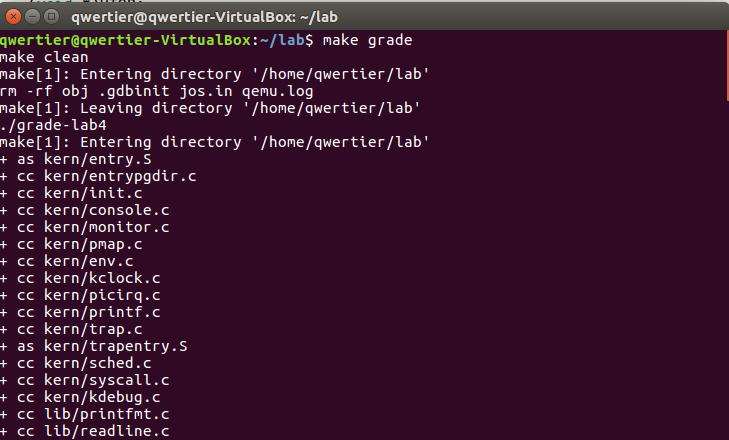
\includegraphics[width=6in]{figures/lab4/finish1.png}
  \caption{Lab4完成图}\label{fig:lab4:finish1}
\end{figure}

\begin{figure}[H]
  \centering
  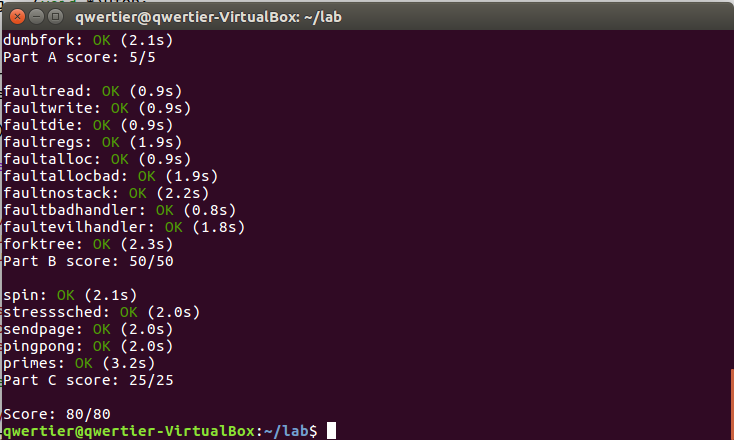
\includegraphics[width=6in]{figures/lab4/finish2.png}
  \caption{Lab4完成图}\label{fig:lab4:finish2}
\end{figure}


\end{ExerciseList}
